\documentclass[UTF8,12pt]{article}
\usepackage{amsmath,amssymb}
\usepackage{pgf,tikz}
\usepackage{pgfplots}
\usetikzlibrary{arrows}
\usepackage{xcolor}

\begin{document}

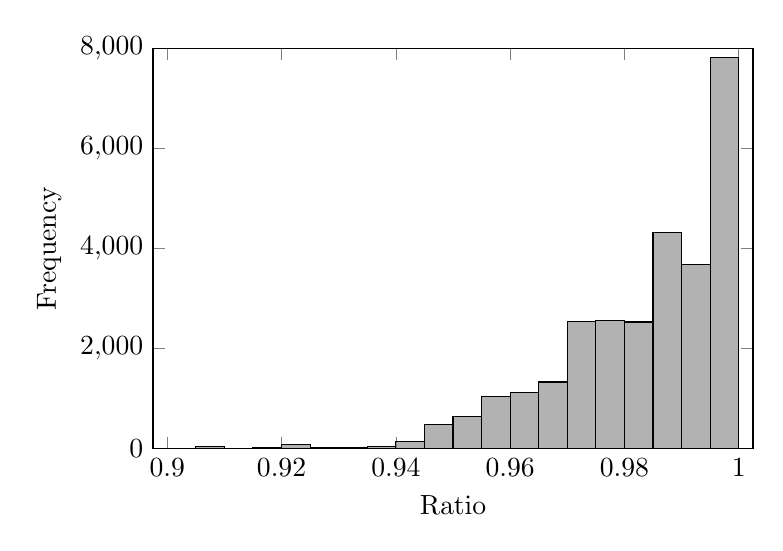
\begin{tikzpicture}

\begin{axis}[%
width=3in,
height=2in,
scale only axis,
xmin=0.8975,
xmax=1.0025,
ymin=0,
ymax=8000,
xlabel={Ratio},
ylabel={Frequency},
axis background/.style={fill=white},
legend style={legend cell align=left, align=left, draw=white!15!black}
]
\addplot[ybar interval, fill=gray, fill opacity=0.6, draw=black, area legend] table[row sep=crcr] {%
x	y\\
0.9	1\\
0.905	40\\
0.91	0\\
0.915	10\\
0.92	81\\
0.925	9\\
0.93	25\\
0.935	43\\
0.94	138\\
0.945	473\\
0.95	635\\
0.955	1039\\
0.96	1125\\
0.965	1329\\
0.97	2547\\
0.975	2558\\
0.98	2530\\
0.985	4319\\
0.99	3686\\
0.995	7812\\
1	7812\\
};

\end{axis}
\end{tikzpicture}

\end{document}